
La premi�re partie est de consuitre les topologies virtualis�es et de
tester les performances de MTPCP en faisant varier les param�tres des
sous-flots. La seconde partie est de construire un alogrithme
d'ordonnancement r�pondant � des crit�res de s�curit�.
\vspace{0.5cm}

Les �tapes du d�veloppement suivront les points suivants:

\begin{itemize}
\item Pr�paration d'une machine mininet avec le noyau MPTCP compil�
  pour l'ensemble de l'�quipe:
\item Lecture, compr�hension et commentaires du code de MPTCP;
\item Pr�paration de plusieurs topologies : \emph{fat tree} pour
  simuler un \emph{data center} et une topologie permettant de tester
  la concurrence entre MPTCP et TCP;
\item Pr�paration d'une biblioth�que de tests et de mesures via l'API python;
\item \'Ecriture d'un algorithme d'ordonnancement dans le noyau;
\item Mesures de performance des diff�rents algorithmes.
\end{itemize}




\begin{figure}[!htb]
  \begin{changemargin}{-2.0cm}{0.5cm}
    \centering
    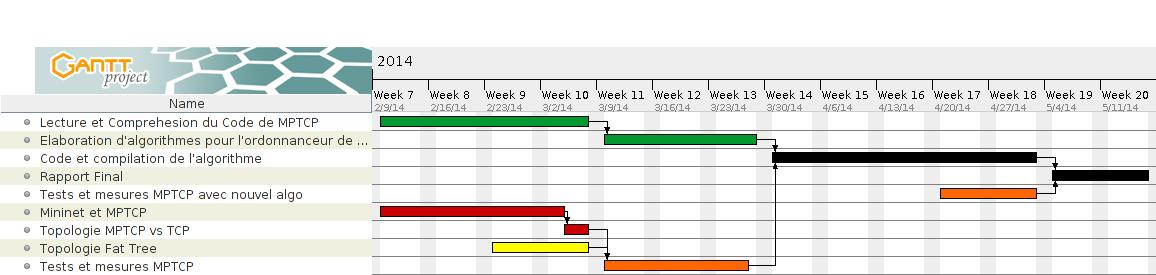
\includegraphics[width=1.2\textwidth]{../gantt/gant.jpg}
  \end{changemargin}
  \centering
  
  \caption{\textbf{Diagramme de Gantt g�n�ral}. Les couleurs
    correspondent � la r�partition entre les membres de l'�quipe : en
    \emph{rouge} M. Ly, en \emph{jaune} M. Ravier et en \emph{vert}
    M. Dubois et M. Lam, en \emph{orange} M. Ravier et M. Ly et en
    \emph{noir} par tout le monde.}
  \label{fig:gantt}
  
\end{figure}

\vspace{2cm}

\begin{figure}[!htb]
  \begin{changemargin}{-2.0cm}{0.5cm}
    \centering
    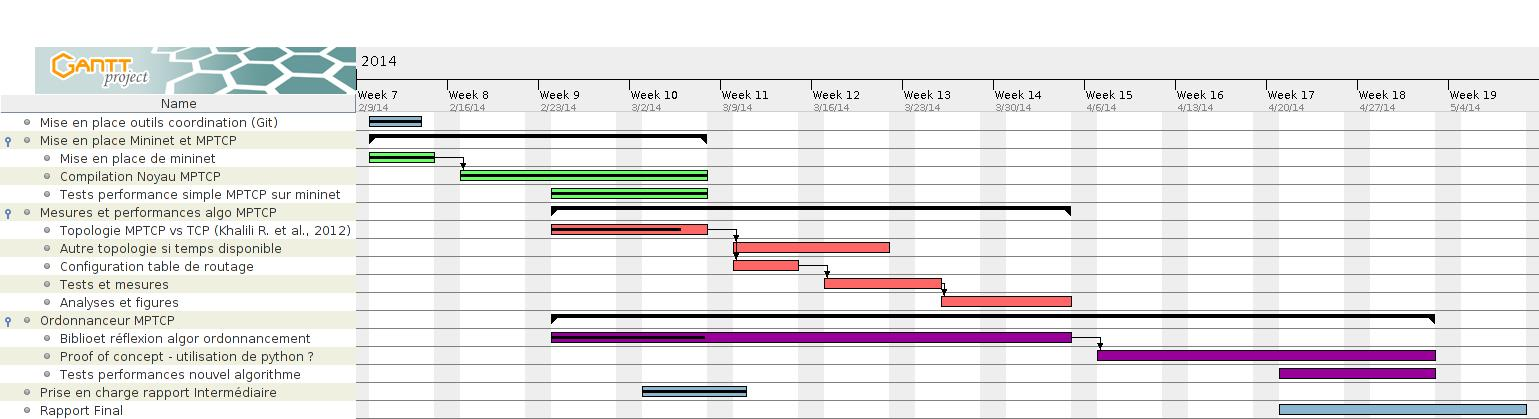
\includegraphics[width=1.2\textwidth]{../gantt/romain.jpg}
  \end{changemargin}
  \centering
  
  \caption{\textbf{Diagramme de Gantt personnalis�e Romain Ly.}}
  \label{fig:gantt}
  
\end{figure}

\begin{figure}[!htb]
  \begin{changemargin}{-2.0cm}{0.5cm}
    \centering
    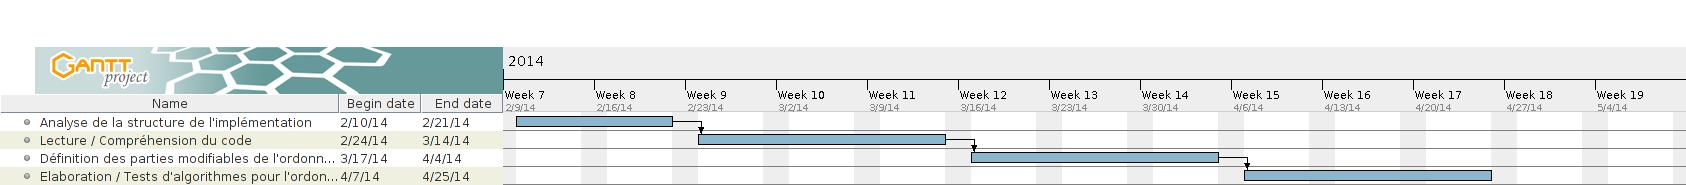
\includegraphics[width=1.2\textwidth]{../gantt/kevin.jpg}
  \end{changemargin}
  \centering
  
  \caption{\textbf{Diagramme de Gantt personnalis�e Kevin Lam et
      Quentin Dubois.}}
  \label{fig:gantt}
  
\end{figure}

